\documentclass[11pt, a4paper, titlepage]{article}

% Set document dimensions
\usepackage[paper=a4paper,top=2cm,left=1.8cm,right=1.8cm,bottom=2cm, includefoot]{geometry}
\usepackage{float}
\usepackage[final]{pdfpages} % inludesvg

\usepackage{listings}

% Czech fonts
\usepackage[T1]{fontenc}
\usepackage[utf8]{inputenc}
\usepackage[czech]{babel}
\usepackage{fancyhdr}


\usepackage{background}
\setlength{\headheight}{3em} 
\newcommand{\subsectionbreak}{\clearpage}

\begin{document}
	\begin{titlepage}
    % \newgeometry{top=1in,top=2cm,left=2cm,right=2cm,bottom=2cm}

    \centering

    {\fontsize{20pt}{15pt}\bfseries
    VYSOKÉ UČENÍ TECHNICKÉ V~BRNĚ\\
    \vspace{8pt}
    Fakulta informačních technologií
    }


    
\includegraphics[scale=0.7]{./assets/fit-logo.pdf}

    \vspace{22pt}

    {\Large Přiručka k aplikaci do předmětu IVS\\}
    \vspace{40pt}
    {\Large \bfseries Super Science Calculator\\}
    
    \begin{figure}[h]
    \centering
    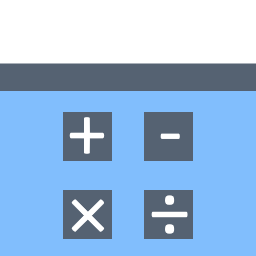
\includegraphics[scale=0.5]{./assets/icon.png}
    \end{figure}
    \vspace{10pt}
    {\Large \today}

    \vspace{90pt}
    {\Large \bfseries Autoři\\}
    \vspace{12pt}

    \begin{tabular}{ l c r }
        Martin Kobelka & \texttt{xkobel02} \\
        Karpíšek Jakub & \texttt{xkarpi06} \\
        Havlín Jan & \texttt{xhavli47} \\
        Vavro Ján & \texttt{xvavro05} \\
    \end{tabular}\\

\end{titlepage}
	\pagestyle{fancy}
	\lhead{\emph{Příručka k aplikaci do předmětu IVS}}
	\rhead{\emph{VUT FIT IVS 2017/2018}}
	\lfoot{\emph{VUT FIT - IVS}}
	\rfoot{\emph{Tým CodeIT@FIT}}

	\begin{center}
		\section*{Uživatelská příručka}
	\end{center}

	\tableofcontents

	\section{Úvod}
	Následující dokument je uživatelskou příručkou k aplikaci super science calculator. Jedná se o projekt do
	předmětu IVS na FIT VUT vyučovaném v letním semestru akademického roku 2017/2018. kalkulačka nabízí 
	plnohodnotné matematické operace, systém proměnných včetně jejich závislostí a blokací smyček i základní podporu
	pro definování uživatelských funkcí.

	Aplikace je napsána v programovacích jazyích \texttt{Java} a \texttt{JavaSctript}. Je částečně pokryta jednotkovými testy.
	grafická vrstva aplikcace byla postavena ve frameworku \texttt{JavaFX}

	\section{Instalace}

	Instalaci je možno provést dvěma způsoby.

	\begin{enumerate}
		\item Za pomocí instalátoru pro operační systém windows, který je dostupný v adresáři install/ windows.
		Windows je zároveň hlavní platformou, pro kterou byla aplikace vyvíjena. Instalace probíhá spuštěním
		souboru \texttt{advanced-science-calculator-1.0-setup.exe}. Spustí se standartní instalátor.
		Po spuštění aplikace může být uživatel vyzván k instalaci platformy java. 
		Odinstalace probíhá spuštěním souboru \texttt{unist000.exe}

		\item Linux je pouze sekundární platformou, a proto obsahuje pouze jednoduchý instlační script \texttt{install.sh}
		pro zkopírování souborů do složky \texttt{/usr/local/lib} a vytvoření souštěče v \texttt{/usr/local/bin}
		V případě, že je script spuštěn s parametrem \textt{-d}, tak se script pokusí vytvořit spustitelného
		zástupce na ploše. Pokud není plocha dostupná, nestane se nic.
		Odinstalace probíhá spuštěním scriptu \texttt{unistall.sh}, který snaže vytvořneé soubory. Ruční odinstalace je možná
		smazáním souborů z výše zmíněných složek, případě zástupce z plochy.
	\end{enumerate}

	\section{Uživateslké rozhraní}

	\subsection{Základní uživatelské rozhraní}

	Uživatelské rozhraní se kládá z několika částí

	\begin{enumerate}
		\item Klávesnice pro zadávání zadávání hodnot myší / dotekem
		\item Vstupní textové pole pro výraz
		\item Odmazání jednoho znaku
		\item vyvolání výpočtu
		\item vizualizace výsledku
		\item Tabulka proměnných
		\item tabulka funkcí
		\item Vyvolání nastavení
		\item Vyvolání nápovědy
		\item Vyvolání informačního dialogu \texttt{about}
	\end{enumerate}

	Tlačítko uživatelé je neaktivní. V současné verzi nebyla tato funkce dokončena, chystá se v budoucí verzi.

	\begin{figure}[t!]
	    \centering
	    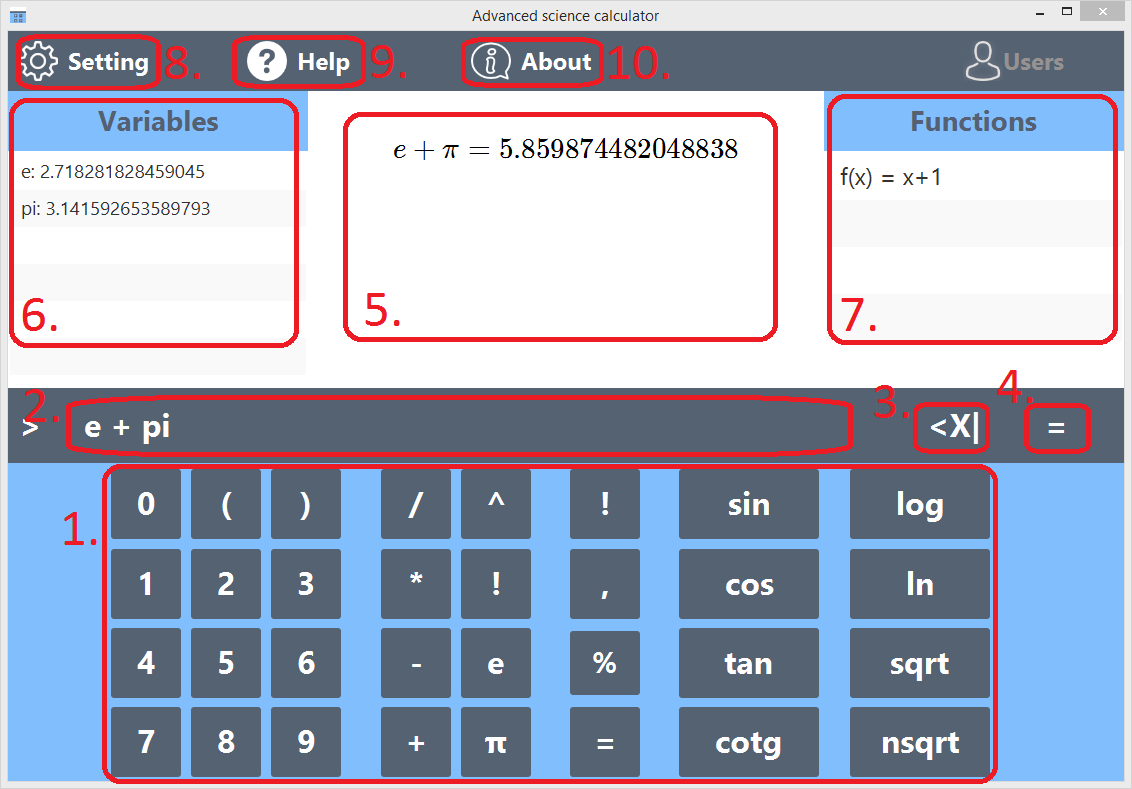
\includegraphics[scale=0.5]{./assets/rozhr.png}
	\end{figure}

	\section{Ovládání aplikace}

	Veškteré ovládání je možné provádět za pomocí několika základních příkazů v textovém políčku 2

	\newpage

	\subsection{Standartní funkce}

	Po zadání libovolného výrazu do textového políčka dojde 2. dojde k parsování a interpret se pokusí
	o provedení výpočtu.

	\begin{figure}[h!]
	    \centering
	    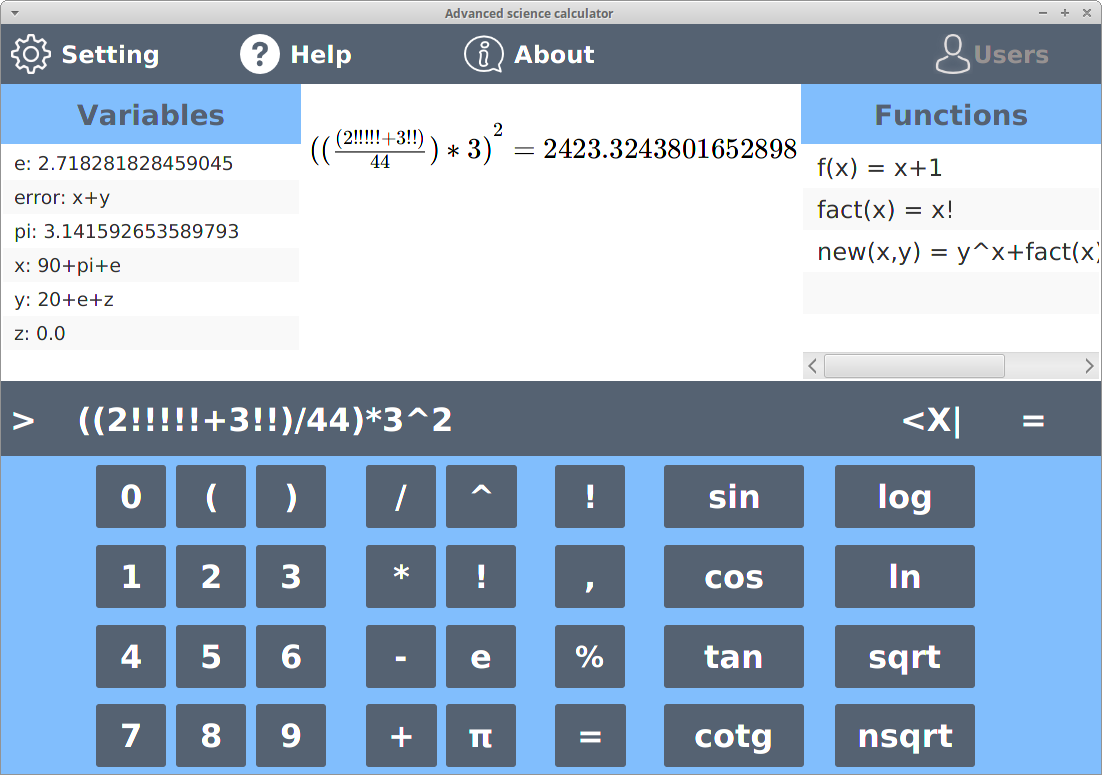
\includegraphics[scale=0.3]{./assets/screenshot.png}
	\end{figure}

	V případě, kdy dojde k dělení nulou, je zadáno ne-celé číslo do operací \texttt{modulo} či \texttt{faktoriál},
	bude výsledek nastaven na hodnotu 0 a uživatel bude upozorněn. V případě zcela nerozpoznatelného výrazu bude
	uživatel buďto upozorněn, nebo bude vykreslení přerušeno do té doby, dokud nebude zadán korektní výraz.

	\begin{figure}[h!]
	    \centering
	    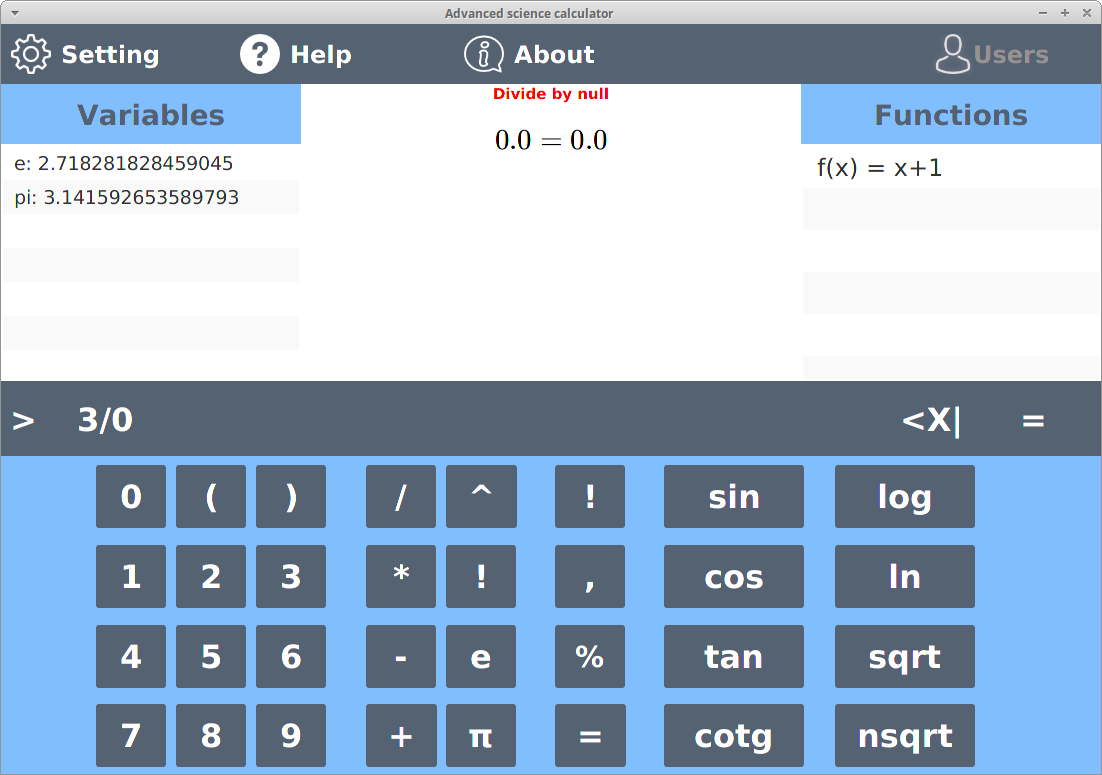
\includegraphics[scale=0.3]{./assets/null.png}
	\end{figure}

	\newpage

	\subsection{Proměnné}

	Proměnné jsou definovány automaticky při prvním použítí, a jejich hodnota je automaticky inicializována na
	hodnotu 0. Zěnit hodnotu je možné za pomocí přiřazovacího příkazu, jehož syntaxe je. K uložení hodnot
	proměnných dochází až po tzv. \texttt{tvrdém potvrzení}, které lze vyvolat stiknutím klávesy 
	\texttt{enter}, nebo kliknutím na tlačítko 4}. Toto si neplést s tlačítkem níže, které znak \texttt{=} vloží
	do textového pole.

	Proměnnou je možné smazat kliknutí a stisknutím klávesy \texttt{delete}. Před smazáním vestavěné proměnné je
	uživatel upozorněn.

	\begin{lstlisting}
	<identifier> = <expression>
	\end{lstlisting}

	\begin{figure}[h!]
	    \centering
	    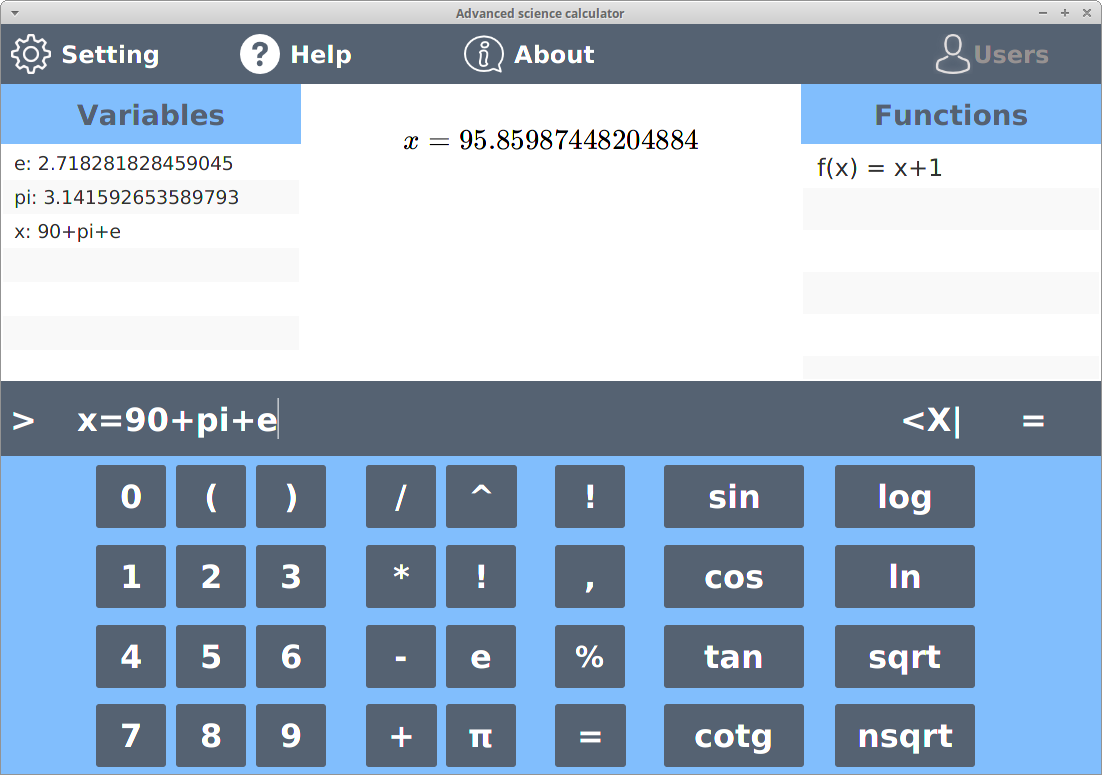
\includegraphics[scale=0.3]{./assets/var.png}
	\end{figure}

	Mezi proměnnými je možné vytvářet libovolně složité závisloti. Závislosti však nesmí tvořit cyklus. V takovém
	případě nebude vytvoření takové proměnné povoleno.

	\begin{figure}[h!]
	    \centering
	    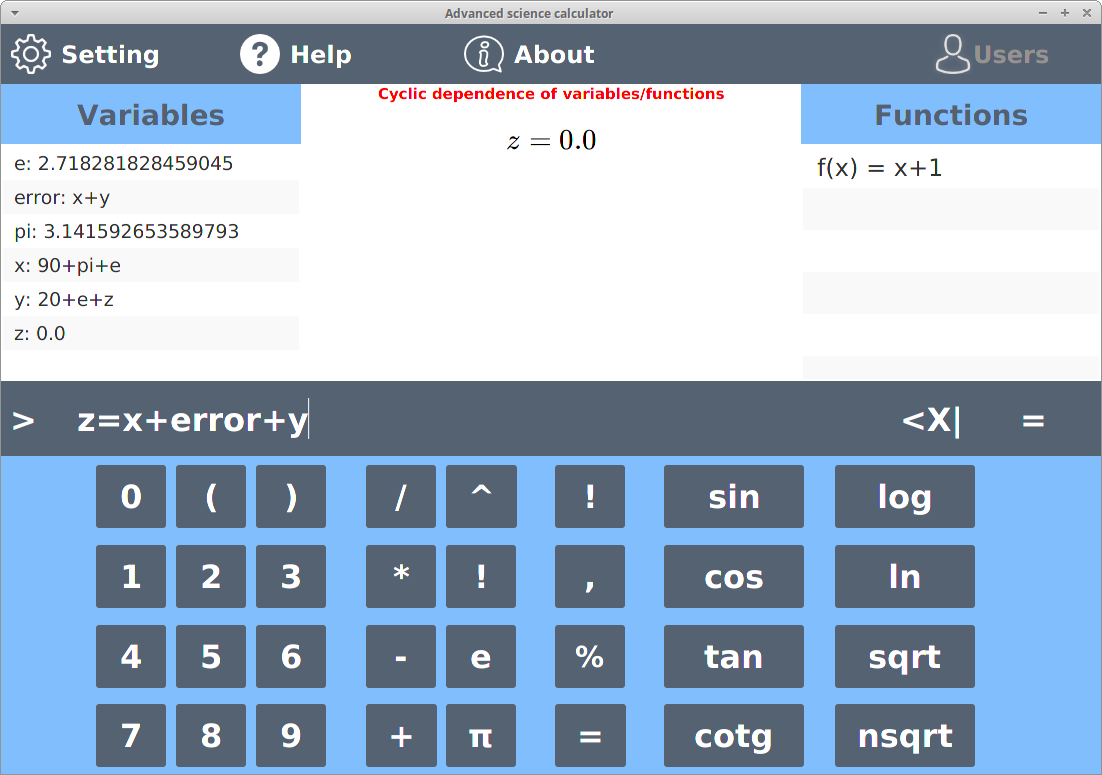
\includegraphics[scale=0.3]{./assets/cycle.png}
	\end{figure}

	\newpage

	\subsection{funkce}
	Funkce je možné definovat za pomocí příkazu s následující syntaxí.

	\begin{lstlisting}
	<identifier>(<argument>,[<arguments>]) = <expression>
	\end{lstlisting}

	funkce taktéž nemohou tvořit závisloti. K zavolání funkce poté může dojít kdekoliv ve výrazu. Chybějící
	argumenty jsou automaticky doplněny na hodnotu \texttt{0.0}

	Pokud některé argumenty funkce nejsou zadány, je automaticky použita hodnota 0.

	Funkce je možné mazat kliknutím a stiknutím klávesy delete. Mezi funkcemi lze z implementačních důvodů vytvářet
	cyklické závislosti, ale není možné takto vytvořené funkce poté volat. (Uživatel bude upozorněn chybovou 
	hláškou)
	
	\begin{figure}[h!]
	    \centering
	    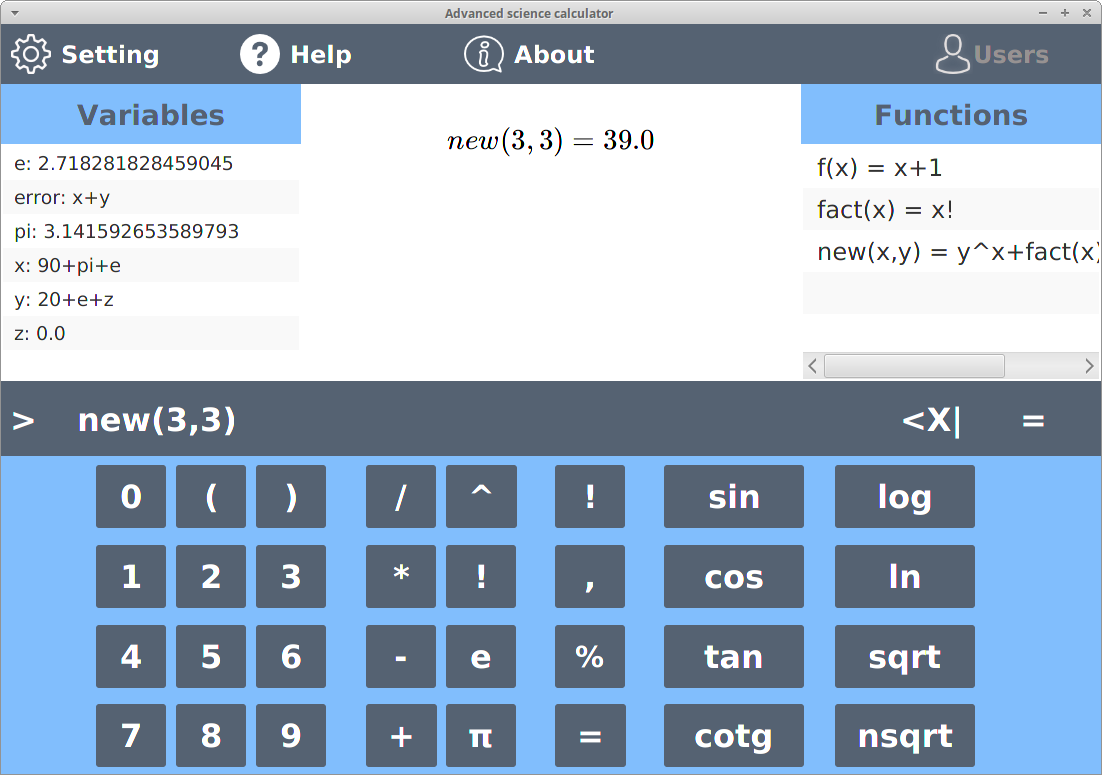
\includegraphics[scale=0.3]{./assets/func.png}
	\end{figure}


	Specialitou funkcí jsou tzv. \texttt{vektorové operace}. Pokud je funkci zadáno více argumentů, zpracuje 
	stejnou operaci s více hodnotami, a vrátí všechny. Takto vytvořené hodnoty je možno dále vnořovat.
	
	
	\begin{figure}[h!]
	    \centering
	    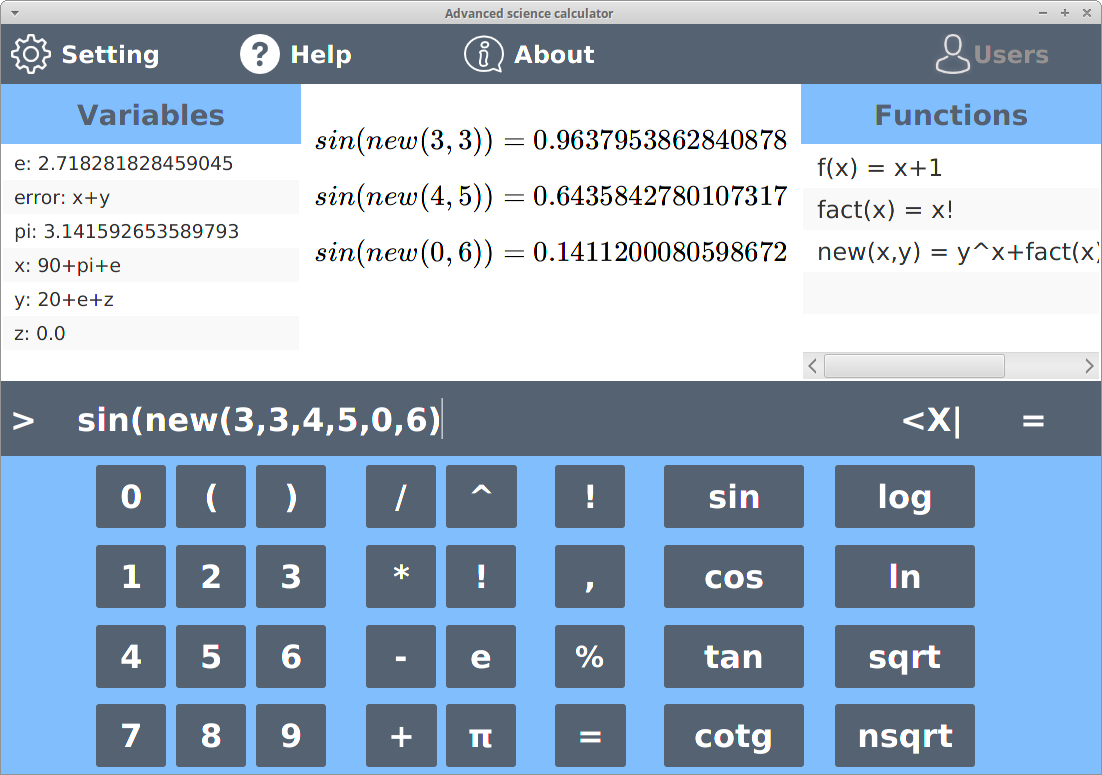
\includegraphics[scale=0.3]{./assets/vector.png}
	\end{figure}

	\newpage
	Všechny hodnoty v kalulačce jsou datového typu vektor. Vektor se vytváří za pomocí operátoru \texttt{,}

	\begin{figure}[h!]
	    \centering
	    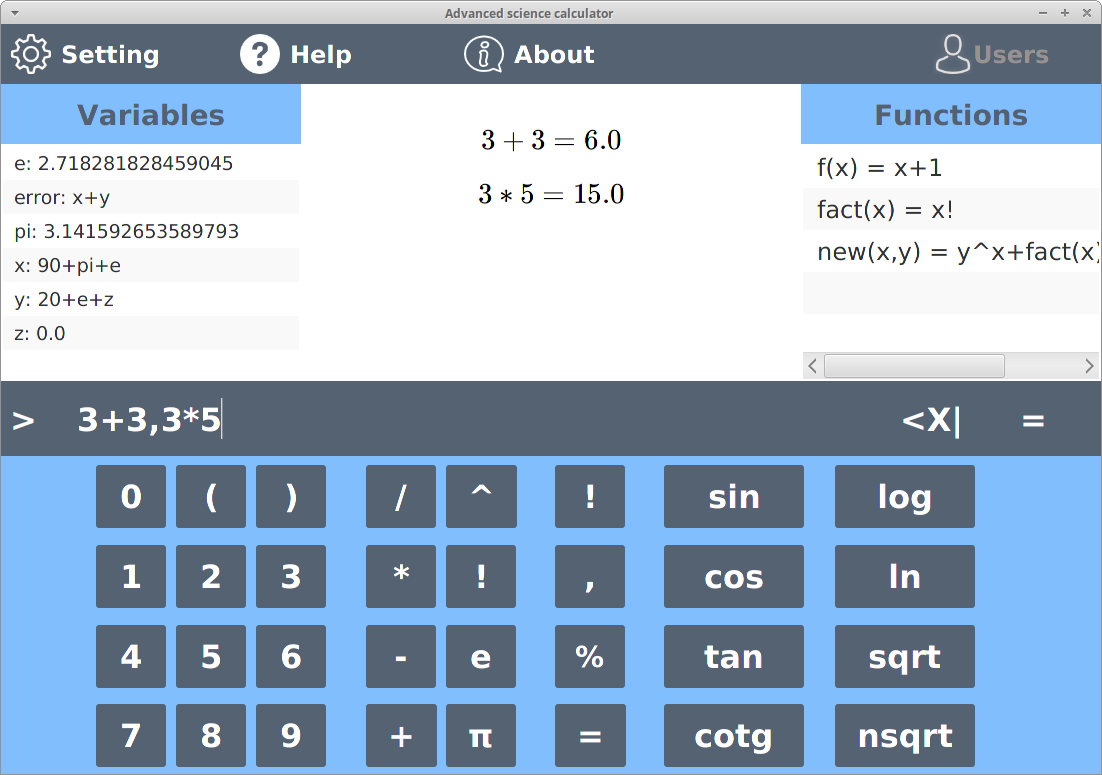
\includegraphics[scale=0.3]{./assets/st_vect.png}
	\end{figure}

	\subsection{vestavěné funkce}

	Kalkulačka disponuje osmi vestavěnými funkcemi. Všechny až na funkci nsqrt (n-tá odmocnina) mají 
	jeden argument (pokud nepracují vektorově). Funkce nsqrt přijimá dva argumenty a počítá n-tou odmocninu
	(první argument) z daného čísla (druhý argument).

	\section{Nastavení}

	Po kliknutí na tlačíko 8 dojde k vyvolání nastavení. Můžeme nastavít několik různých aspektů. Všechny aspekty jsou perzistentní, a po
	jejich změně dojde k automatickému nastavení.
	 
	\begin{figure}[h!]
	    \centering
	    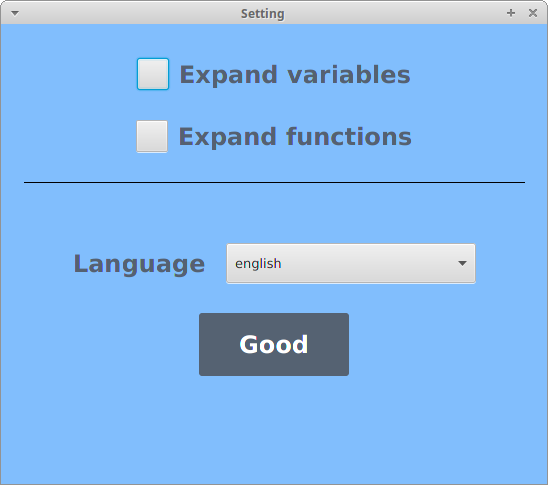
\includegraphics[scale=0.5]{./assets/set.png}
	\end{figure}

	Jazyky jsou uloženy velde aplikace každý v jenom *.xml souboru. Uživatel může bez znalosti programování
	vytvářet jazyky nové. Ovšem aplikace \textbf{nemůjde bez složky languages spustit}.

	\subsection{expanze proměnných / funkcí}

	Po zaškrtutí těchto políček budou všechny proměnné ve vykreslovacím režimu expandovány až na čísla.
	Stejnou akci lze provádět u funkcí. U funkcíc to ovšem nemusí vždy fungovat spolehlivě, jelikož
	výraz zadaný jako argument může být z implementačních důvodů převeden na číslo,
	a provedené operace se mohou ztratit. Ne však hodnota. Honnota 
	\textbf{zůstává při zapnuté i vypnuté expanzi stejná}

	\subsubsection{Při vypnuté expanzi}
	
	\begin{figure}[h!]
	    \centering
	    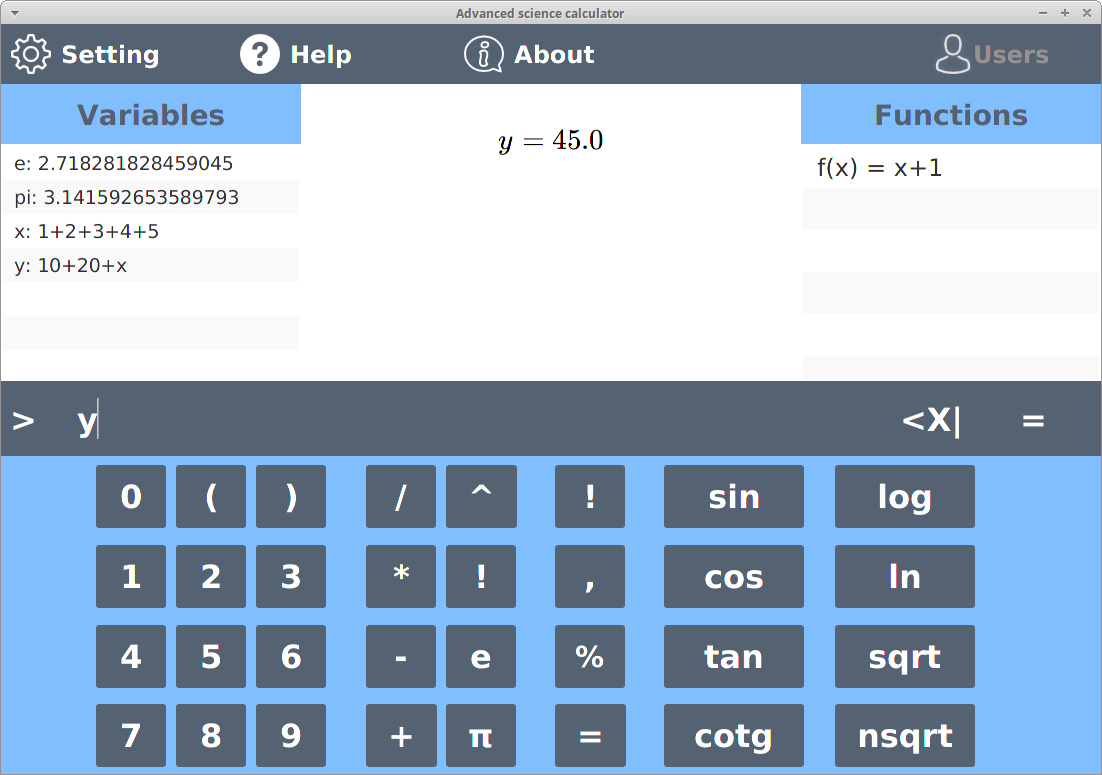
\includegraphics[scale=0.25]{./assets/expof.png}
	\end{figure}

	\subsubsection{Při zapnuté expanzi}

	\begin{figure}[h!]
	    \centering
	    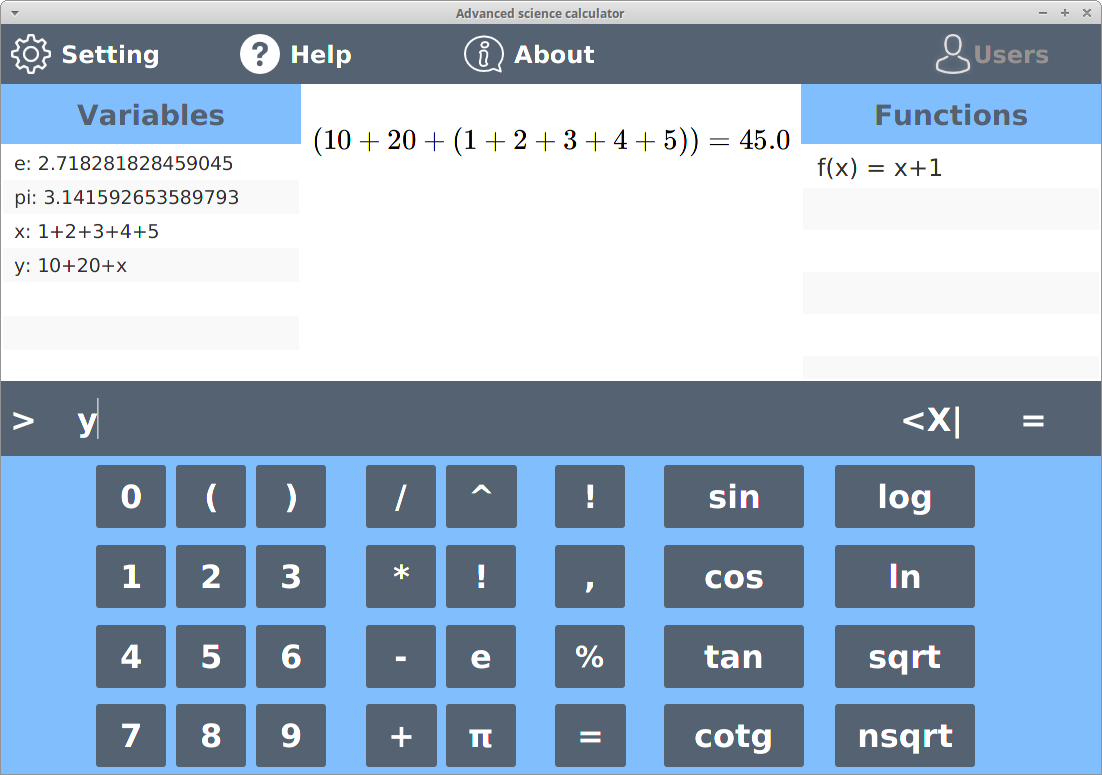
\includegraphics[scale=0.25]{./assets/expon.png}
	\end{figure}

	\newpage

	\section{Práce v příkazové řádce}

	Kalkulačku je možné použít i v režimu příkazové řádky. Tento režim není příliš propracován,
	ale interpret se v takovém případě pokusí zpracovávat vámi zadávané příkazy stejně, jako kdyby 
	byly zadávány do textového pole.

	Režim příkazové řádky je vyvolán po spustění s paramenterm \texttt{--cli} nebo \texttt{-c}.

	\begin{figure}[h!]
	    \centering
	    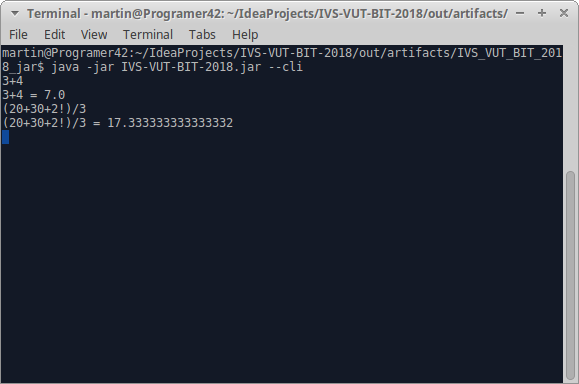
\includegraphics[scale=0.8]{./assets/cli.png}
	\end{figure}

	\subsection{Profiling}

	Aplikaci pro výpočet směrodatné odchylky je možné spustit, pokud aplikaci spustíme s parametrem
	\texttt{--profiling} nebo \texttt{-p}. ČÍsla se možné zadávat oddělené čárkami a nebo konci řádku.
	Dvě čísla však nemohou být oddělemi i čárkou i koncem řádku.

	\subsection{Pomoc}

	Po spuštění apliakce s parametrem \texttt{--help} nebo \texttt{-h} dojde k vyvolání matuálu pro 
	spuštění aplikace.
	

\end{document}
